%-----------------------------------------------------------------------------
%
%               Template for sigplanconf LaTeX Class
%
% Name:         sigplanconf-template.tex
%
% Purpose:      A template for sigplanconf.cls, which is a LaTeX 2e class
%               file for SIGPLAN conference proceedings.
%
% Guide:        Refer to "Author's Guide to the ACM SIGPLAN Class,"
%               sigplanconf-guide.pdf
%
% Author:       Paul C. Anagnostopoulos
%               Windfall Software
%               978 371-2316
%               paul@windfall.com
%
% Created:      15 February 2005
%
%-----------------------------------------------------------------------------


\documentclass[10pt]{sigplanconf}

% The following \documentclass options may be useful:

% preprint      Remove this option only once the paper is in final form.
% 10pt          To set in 10-point type instead of 9-point.
% 11pt          To set in 11-point type instead of 9-point.
% authoryear    To obtain author/year citation style instead of numeric.

\usepackage{amsmath}


\usepackage{graphics} % for EPS, load graphicx instead 
%\usepackage[T1]{fontenc}
\usepackage{txfonts}
\usepackage{times}    % comment if you want LaTeX's default font
\usepackage[pdftex]{hyperref}
% \usepackage{url}      % llt: nicely formatted URLs
\usepackage{color}
\usepackage{textcomp}
\usepackage{booktabs}
\usepackage{ccicons}
\usepackage{todonotes}
\usepackage{tabularx}
\usepackage{listings}
\usepackage[utf8]{inputenc}
\usepackage{realboxes}


\definecolor{c0}{HTML}{FC3332}
\definecolor{c1}{HTML}{D13094}
\definecolor{c2}{HTML}{A444FB}
\definecolor{c3}{HTML}{4256FB}

\definecolor{c4}{HTML}{178AFB}
\definecolor{c5}{HTML}{23CCF5}
\definecolor{c6}{HTML}{31E529}
\definecolor{c7}{HTML}{ABE22D}

\definecolor{c8}{HTML}{BEBC27}
\definecolor{c9}{HTML}{FED130}
\definecolor{c10}{HTML}{FDA12B}
\definecolor{c11}{HTML}{FC6827}


\definecolor{codebackground}{rgb}{0.97,0.97,0.97}
\definecolor{linenumbers}{rgb}{0.25,0.25,0.25}
\definecolor{keywordcolor}{rgb}{0.1,0.1,0.6}
\definecolor{commentcolor}{rgb}{0.1,0.5,0.1}

\lstdefinelanguage{lidl}
{
 keywords={in, out, type, interface, interaction, is ,with, ref},
 sensitive=false,
 morecomment=[l]{//},
 morecomment=[s]{/*}{*/},
 morestring=[b]",
}

\lstset{
 language=lidl,
 basicstyle=\ttfamily\footnotesize,            % print whole listing small
 keywordstyle=\color{keywordcolor}\bf\ttfamily,% underlined bold black keywords
 tabsize=2,                    % sets default tabsize to 2 spaces
 captionpos =b                 % sets the caption-position to bottom
 keepspaces = true,             % keeps spaces in text
 % identifierstyle=,           % nothing happens
 commentstyle=\color{commentcolor}\textit,         % white comments
 stringstyle=\ttfamily,        % typewriter type for strings
 showstringspaces=false,       % no special string spaces
 %columns=flexible,             % colonnes "flexibles"
 basewidth={0.5em},           % dimension des colonnes
 fontadjust=true,              % pour ajuster les polices
 breaklines=true ,             % pour le retour à la ligne dans les colonnes
 backgroundcolor=\color{codebackground},
 numbers=left,                    % where to put the line-numbers; possible values are (none, left, right)
 numbersep=5pt,                   % how far the line-numbers are from the code
 numberstyle=\tiny\color{linenumbers}, % the style that is used for the line-numbers
}

%\newcommand{\code}[1]{\Colorbox{codebackground}{\lstinline{#1}}}
\newcommand{\code}[1]{\lstinline{#1}}



\begin{document}

\special{papersize=8.5in,11in}
\setlength{\pdfpageheight}{\paperheight}
\setlength{\pdfpagewidth}{\paperwidth}

\conferenceinfo{SLE '15}{Month d--d, 20yy, City, ST, Country} 
\copyrightyear{20yy} 
\copyrightdata{978-1-nnnn-nnnn-n/yy/mm} 
\doi{nnnnnnn.nnnnnnn}

% Uncomment one of the following two, if you are not going for the 
% traditional copyright transfer agreement.

%\exclusivelicense                % ACM gets exclusive license to publish, 
                                  % you retain copyright

%\permissiontopublish             % ACM gets nonexclusive license to publish
                                  % (paid open-access papers, 
                                  % short abstracts)

\titlebanner{banner above paper title}        % These are ignored unless
\preprintfooter{short description of paper}   % 'preprint' option specified.

\title{The LIDL Interaction Description Language}
\subtitle{A language for the description of interaction}

\authorinfo{Vincent Lecrubier }
           {ONERA DTIM/LAPS}
           {lecrubier@onera.fr}
\authorinfo{Bruno d'Ausbourg}
           {ONERA DTIM/LAPS}
           {ausbourg@onera.fr}
\authorinfo{Yamine A\"it-Ameur}
           {ENSEEIHT}
           {yamine@enseeiht.fr}


\maketitle

\begin{abstract}
This paper describes LIDL, a language dedicated to the specification of interactive systems. LIDL is based on the idea that most programming languages are useful to specify computations, but are not adequate when it comes to specifying interactions. We first introduce the context and the need for new paradigms for interactive systems specification. Then we describe the basic concepts of LIDL, such as Interfaces, Data activation, Interactions, and LIDL program structure an syntax. Some uses of LIDL programs such as verification, code generation and automated testing are then explained. Finally, an interactive system is partially developed using LIDL, as an example use case.
  \end{abstract}

\category{H.5.m.}{Information Interfaces and Presentation
  (e.g. HCI)}{Miscellaneous} 

\keywords{Human-Machine Interfaces; Domain-Specific Language; Interactive Systems; Formal Language; Critical Systems}


%%%%%%%%%%%%%%%%%%%%%%%%%%%%%%%%%%%%%%%%%%%%%%%%%%%%%%%%%%%%%%%%%%%
\section{Introduction}


\subsection{Aeronautical background}

A lot  of research  work have  focused on how  to design,  program and
verify functional concerns for  critical systems and more particularly
aeronautical  systems.  HMI   systems  did   not   benefit  from   the
same  attention   and efforts. 

A significant  amount of work has  focused on devising models  for the
development  process of  software  systems in  the  field of  software
engineering.

The system development  process in critical domains  as, for instance,
in aeronautics  inherited these  models.  This  process is  now widely
based on  the use of standards  that take into account  the safety and
security  requirements   of  the   systems  under   construction.   In
particular the DO178C  standard \cite{DO178C}, in aeronautics, defines
very strict  rules and instructions  that must be followed  to produce
software  products,  embedded  systems   and  their  equipments.   The
objective is to ensure that the  software performs its function with a
safety level in accordance with the safety requirements.

Because of the problem stated in Figure \ref{fig:twoClashingDomains}, the HMI development does not  follow the same processes. Nevertheless,
in aeronautics, HMI  systems are now made up by  multiple hardware and
software components embedded in  aircraft cockpits.  These systems are
large and complex artifacts that  also face tough constraints in terms
of  usability,   security  and   safety.   They   support  interactive
applications  that must  behave  as  intended with  a  high degree  of
assurance  because  of their  criticity.   An  error in  the  software
components that implement interactions  in these applications may lead
to a human or system fault that may have catastrophic effects.  


For example, the BEA report \cite{BEA12} about the crash of Rio-Paris AF-447 
A330 Airbus establishes that,  during the flight, interface system
displayed some actions to be performed by the pilot in order to change
the pitch  of the aircraft  and to nose it  up while it  was stalling.
These indications should clearly not  have been displayed.  Indeed, by
following those  erroneous displayed instructions the  pilot increased
the stalling of the aircraft.

In  fact,  in  the  industrial context,  the  development  process  of
critical interactive  embedded applications stays very  primitive. The
usual  notations  are  essentially  textual and  coding  is  generally
performed  from  scratch or  by  reusing  previous developments  based
themselves  on textual  specifications. In  aeronautics, the  produced
code must be in  conformance with the ARINC~661 standard \cite{ARINC661}.
It may  be noticed that  some tools  recently appeared to  enhance the
design and  coding stages of these  systems.  But these tools,  as for
instance   Scade  Display \cite{scade-display},  deal   mainly   with
presentation layers of the systems and  do not deal with their complex
functional behaviour. In  this context, the validation  process of the
interactive  applications  is  very  restricted and  poor  because  it
resides practically  only in  a massive test  effort and  in expensive
evaluation phases  at the  end of  the development  process.  Moreover
there is no actual formal reference  to check the implementation is in
conformance with. So new approaches and new paradigms are today needed
to help  in the development  process of critical  interactive embedded
applications.



\begin{figure}[h]
\centering
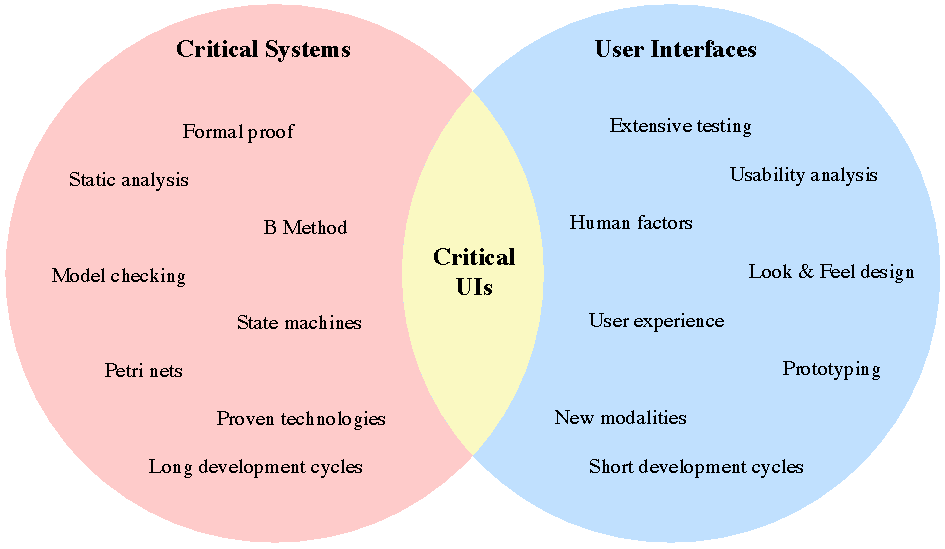
\includegraphics[width=\linewidth,height=\linewidth,keepaspectratio]{figures/twoClashingDomains.pdf}
\caption{Critial UIs development is as the intersection of two clashing domains.} 
\label{fig:twoClashingDomains}
\end{figure}

\subsection{Generalization}

During the development of LIDL, we realised that the ideas developed in LIDL could also be used successfully to describe other non-critical interactive systems. Indeed, many fields lack appropriate ways to describe interactive systems. 

In the field of desktop applications, almost all the popular user-interface toolkits and libraries rely on imperative or object-oriented languages. This means that developers have to use objects in order to describe interactive systems. For instance, Qt or Java programmers are familiar with the notion of listeners, observer, signals, slots... These object-oriented approaches are powerful, but they tend to lead to complex code, sometimes called \emph{spaghetti code} when the complexity becomes intractable.

As expressed in \cite{chatty2007}, most of the time, developers would like to specify interactions they want their program to perform. But  instead, they end up having to code programs that describe how to create and connect groups of objects (widgets, listeners...) that will perform the intended interaction as an emergent behaviour. This adds a lot of complexity and costs, as well as bugs.
  
The problem is similar in the field of web applications, where many different approaches exists in order to tackle the complexity, but none seems to be satisfactory, as new approaches are created on a regular basis. Hundreds of frameworks try to solve the problem in different ways, but this is a difficult task. As an example, \cite{todomvc} compiles a list of hundreds of different implementations of the same web application. 

Finally, the emerging internet of things still misses a language which would allow non-programmers to easily express the interaction of smart objects. Companies such as \cite{ifttt} have devised ways for the general public to describe simple interactions they want their connected objects to perform, but the expressive power of the pseudo-language used is very restrictive.

Overall, it seems that the relative success of general-purpose programming languages in describing interactive systems has eclipsed the urgence of the need for a language specifically designed to describe interactive systems. But as we have seen, the increasing complexity of interactions in a more and more connected digital world is taking general-purpose languages to their limits when it comes to the description of interactive systems.


%\subsection{Similar approaches}
%
%Elm and FRP. LIDL approach is related to functional reactive programming \cite{wan2000functional}. However, LIDL takes a more pragmatic approach to the problem, by simplifying the link between the language semantics and the operational execution.
%
%
%Synchronism from Lustre \cite{halbwachs91}
%
%Typing from JS

%%%%%%%%%%%%%%%%%%%%%%%%%%%%%%%%%%%%%%%%%%%%%%%%%%%%%%%%%%%%%%%%%%%
\section{The LIDL language}

It seems to us that the current state of the art provides no complete solution to the need described in the introduction. The aim of LIDL is to provide a language and tools to deal with this set of problems. LIDL is a relatively simple language based on a small set of features that make sense once put together. The following paragraphs will describe important features that make LIDL a unique language.

\subsection{Interaction-oriented approach}

LIDL programs are defined in a declarative manner, and represent the behaviour of interactive systems whose execution is synchronous, with discrete time steps.

While most programming languages focus on the description of \emph{computations}, the main idea behind LIDL is to describe \emph{interactions}. This is quite a paradigm shift in the sense that many experienced programmers will at first be surprised by the language semantics. However, we argue that LIDL provides an easier way to specify interactive systems, since its main concepts (interfaces and interactions) are more relevant to the field of interactive systems than other programming languages concepts (objects, functions, algorithms...)

A LIDL system represents exactly one interaction. Since interactions can be composed of several simpler interactions connected through interfaces, most non-trivial LIDL programs are a composition of interactions. Actually, LIDL represents everything as interactions. While most programming languages have many different constructions (conditionals, loops, assignments, variables, class declarations, expressions...), LIDL only has two concepts: interactions and interfaces. 

\paragraph{Rationale}

The rationale behind this \emph{interaction-oriented} approach is that LIDL is meant to describe interactive systems. Hence, the only entity that adds value to the description is the interaction. Pushing this interaction-orientation as far as possible led us to the realisation that nothing more than interactions and interfaces is needed, which results in a simple but expressive language.




\subsection{Synchronous execution}

LIDL systems are synchronous. This means that interactions are evaluated at discrete points in time, all at once. As shown in Figure \ref{fig:synchronous}, LIDL systems are similar to state machines. They have a set of input interactions, a set of output interactions, a set of state interactions, and a transition function.

On each step, the transition function uses the previous state and the current input in order to compute the current state and the output of the system.

\begin{figure}[h]
\centering
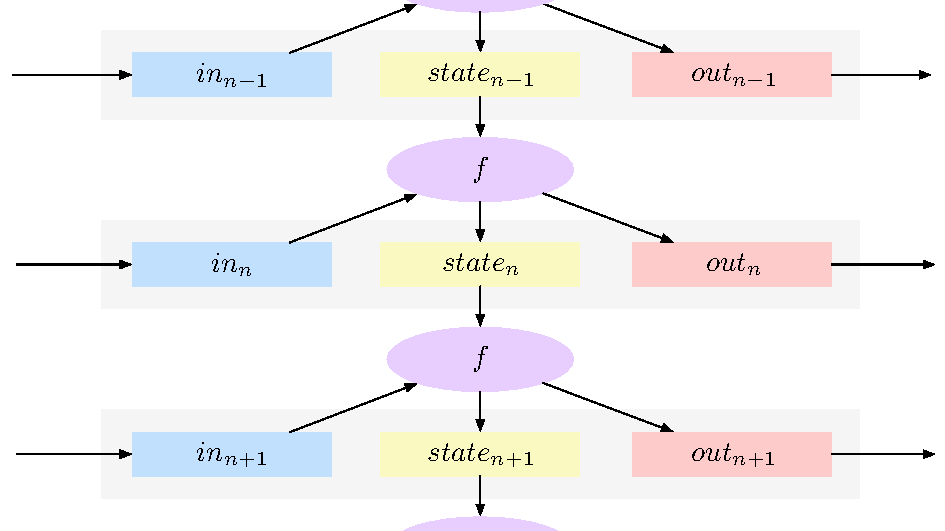
\includegraphics[width=\linewidth,height=\linewidth,keepaspectratio]{figures/synchronous.pdf}
\caption{LIDL systems execution} 
\label{fig:synchronous}
\end{figure}



\paragraph{Rationale}

Synchronous execution tends to simplify the language. The state of the system is explicitly defined for each execution step. This makes reasoning about the code simpler than asynchronous execution. It also maps well to many model checking methods and tools.


\subsection{Interfaces}

An important feature of LIDL is the notion of \emph{interface}. An interface is the combination of two orthogonal aspects: the data type and the data direction. Interfaces are central in LIDL as they have the same role as data types in typed programming languages.

The notion of data type is well known to most programmers. The notion of data direction is also quite easy to understand: the data can either go \emph{in} or go \emph{out}. The notion of interface is hence quite easy to catch, here are a few example of basic interfaces: \code{Number in}, \code{Boolean out}, \code{Text in}...

The same way compound data types exist in other languages, one can express compound interfaces. The syntax to specify compound interfaces is inspired by the Javascript Object Notation (JSON) \cite{jsonstandard}. Listing \ref{exampleinterface} shows an example compound interface defined in LIDL.


\begin{lstlisting}[caption=LIDL definition of the example interface,label=exampleinterface]
interface Example is
  {
    redSquares      : Square in,
    greenPentagons  : Pentagon in,
    yellowTriangles : Triangle out,
    blueCylinders   : Cylinder out
  }
\end{lstlisting}

Metaphorically, interfaces can be seen as the specification of pipes of specific shapes that allow objects to go in specific directions. Figure \ref{fig:interface} shows a way to visualise the example interface of Listing \ref{exampleinterface}.

\begin{figure}[h]
\centering
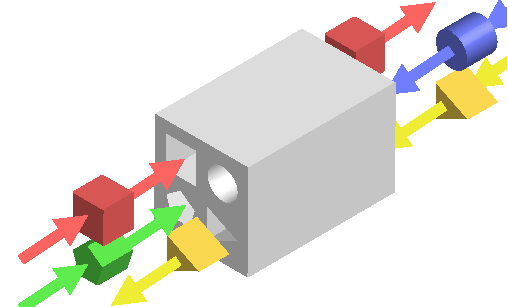
\includegraphics[width=\linewidth,height=\linewidth,keepaspectratio]{figures/interface.pdf}
\caption{A metaphor of LIDL interfaces as pipes that allow specific data types to flow in specific directions } 
\label{fig:interface}
\end{figure}

Every interface has a conjugate interface, which has the same data types, but opposite directions. Two interactive systems can only connect if their interfaces are conjugate. This is the consequence of the natural intuition that the \emph{output} of an entity is the \emph{input} of another one.



\paragraph{Rationale}

Typed programming languages rely on data types to check the composability of functions and operations. This is convenient when the goal is to describe \emph{computations}. But this is not enough when we try to describe \emph{interactions}.  When composing interactions, another very important aspect which is rarely stated explicitly is the \emph{direction} data goes in. 

Most programming languages see data as information \emph{stored} at some places. This makes the answer of several important questions difficult to get. When analysing an interactive program, one can (and should!) ask the following questions: 

\begin{itemize}
  \item Where does this piece of data come from?
  \item What is susceptible of modifying this piece of data?
  \item Which part of the program have access to this piece of data?
  \item Does this reference refer to this piece of data?
\end{itemize}

These questions can become really complex, and are often the cause of many bugs. This is why languages came up with different solutions that allow to answer or simplify these issues: Immutable data types, \code{const} and \code{volatile} keywords in the C language, encapsulation in object-oriented programming languages,...

On the other hand, LIDL sees data as information that \emph{flows} from interactions to interactions. The previous questions hence become trivial, because the programmer always knows where the data comes from, and where it is going.


\subsection{Data activation}


Every piece of data in a LIDL program integrates a notion of activation. The implementation is really simple: \emph{all} LIDL data types are extended with the \emph{inactive} value noted $\bot$. For example, the following table shows example values for the basic data types of LIDL:

\begin{tabularx}{\linewidth}{l|X}
  Type & Example values \\
  \hline
  \texttt{Activation} & $\bot$, $\top$ \\
  \texttt{Boolean} &  $\bot$, $true$, $false$ \\
  \texttt{Number} &  $\bot$, $0$, $1$, $3.14159$ \\
  \texttt{Text} &  $\bot$, $"Foo"$, $"Bar"$, $"Baz"$ \\
\end{tabularx}

Very simplistically, a flow is represented in LIDL by a piece of data which is almost always active. For example, through an execution, a continuous data flow could have the following trace: $\{ 451, 453, 452, 450, 454, ...\}$. On the other hand an event is represented by a piece of data which is almost always inactive. For example, through an execution, an event could have the following trace: $\{ \bot, \bot, \bot, click, \bot, ...  \}$

The notion of activation does not break composability. Here is a compound data type expressed in LIDL : \texttt{\{x:Number,y:Number\}}. This data type is a labelled product data type, similar to a \texttt{struct} of the C language. Here are a few example of values of this type: \texttt{\{x:3,y:2\}}, \texttt{\{x:$\bot$,y:3\}}, \texttt{$\bot$}.





\paragraph{Rationale}

Interactive systems mostly rely on two different paradigms: flow-based representations and event-based representations. 

Flow-based representations maps well to systems whose data is defined on \emph{continuous} time intervals, such as physical measurements for example. Examples of flow-based representations include Lustre \cite{halbwachs91}, Scade... 

On the other hand, event-based systems maps well to systems whose data is defined on discrete time sets, such as clicks on a button. Examples of event-based representations include most User Interface (UI) Toolkits such as Java Swing, Qt...

Several approaches tried to bridge the gap between flow and event representations \cite{abowd22integrating}. However most approaches are biased toward one paradigm or the other. Interestingly, some approaches treat input and output differently, for example by only allowing discrete inputs (events) and continuous output (status). Figure \ref{fig:discreteContinuous} presents the positioning of different academic approaches regarding this aspect. Shown approaches include \cite{halbwachs91}, \cite{dix1991formal}, \cite{Dix85}, \cite{Duke-Harrison93a}, \cite{Harel97}, \cite{actors86}, \cite{Paterno92}, \cite{Navarre:2009:IMU:1614390.1614393} and LIDL.

\begin{figure}[h]
\centering
\includegraphics[width=\linewidth,height=\linewidth,keepaspectratio]{figures/discretecontinuous.pdf}
\caption{Positions of different academic approaches in the flow vs event space.}
\label{fig:discreteContinuous}
\end{figure}

Restriction to a paradigm or the other often prevents natural description of interactive systems, which generally are best described using a mix of both. LIDL proposes a simple way to unify and mix the two paradigms: the notion of data activation.

The notion of data activation is latent in industrial art. Most languages exhibit constructions such as the $null$ value, the $maybe$ monad, callback functions, listeners, observers, signal slots...

In the context of interactive systems, all these constructions boil down to one unique concept: identify the presence of a piece of data, most of the time a message that has to be received or sent. This is exactly what the data activation feature of LIDL does.













\subsection{Interactions}

LIDL is a language to describe interactions. The interaction language has a simple syntax, which uses a lot of parentheses. An interaction is a phrase between parentheses, and it composes trivially. Listing \ref{exampleexpression} shows an example interaction expression, while Figure \ref{fig:example1} shows its structure.

\begin{lstlisting}[caption=An example interaction expression,label=exampleexpression]
(when(not(powered))then(turn(light)red))
\end{lstlisting}

\begin{figure}[h]
\centering
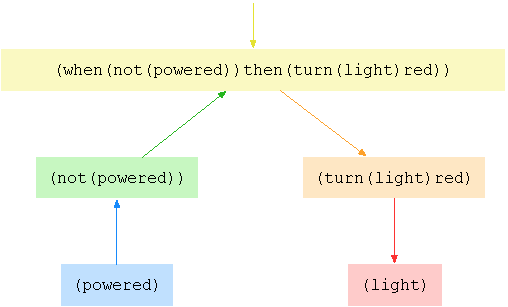
\includegraphics[width=\linewidth,height=\linewidth,keepaspectratio]{figures/example1.pdf}
\caption{The structure of the example expression. Arrows represent the data flow direction} 
\label{fig:example1}
\end{figure}


The semantics of interactions is the most challenging part of LIDL for newcomers, because it is the most disruptive part of the language, since it leverages interfaces and the notion of activation. 

Each interaction (i.e. each pair of parentheses, i.e. each block in Figure \ref{fig:example1}) is attributed a value at each execution step.  Depending of the data direction of the interface of the interaction, this value can be defined by the interaction itself (\code{out}) or by an external interaction (\code{in}). 

Interactions that comply to the \code{out} interface behave like functions. They output a value, based on their arguments. For example \code{(not(powered))} receives a boolean \code{(powered)} and outputs a boolean that is the negation of \code{(powered)}. This is explained in the following table, which should be easy to understand, with parameters on the left column, and results on the right: 

\begin{tabularx}{\linewidth}{X|X}
  \texttt{(powered)}& \texttt{(not(powered))} \\
  \hline
  $true$& $false$ \\
  $false$&  $true$\\
  $\bot$ & $\bot$
\end{tabularx}

Interactions that comply to the \code{in} interface behave the opposite way, which is \textbf{completely foreign} to programmers. Imagine a function that does not \emph{return} a value based on the arguments it receives, but that \emph{receive} a value, and returns values to its arguments. For example \code{(turn(light)red)} receives an activation, and outputs a colour \code{light} which is red when the interaction is active, or $\bot$ the rest of the time. This is summarised in the following table, which will look \textbf{unfamiliar} to most programmers, with parameters on the left column, and computation result on the right:


\begin{tabularx}{\linewidth}{l|X}
  \texttt{(turn(light)red)} &\texttt{(light)} \\
  \hline
  $\top$ & $\{red:255,green:0,blue:0\}$ \\
  $\bot$ & $\bot$ 
\end{tabularx}

The main advantage of LIDL interaction expressions is that they are very general. Many first-class constructions of other programming languages can be represented as LIDL interactions. As an example, the following table quickly summarises the semantics of the \code{()=()} interaction. Note that this interaction complies with the \code{in} interface, indeed, its behaviour consists in sending to the left-hand-side the value it receives on the right-hand-side, \emph{only} when the interaction is active. The control flow, which is implicit in most programming languages, is represented explicitly by the value received by the \code{()=()} interaction.

\begin{tabularx}{\linewidth}{XX|X}
  \texttt{((x)=(y))} & \texttt{(y)}&\texttt{(x)} \\
  \hline
  $\top$ & $5$ & $5$ \\
  $\top$ & $\bot$ & $\bot$ \\
  $\bot$ & $5$ & $\bot$ \\
  $\bot$ & $\bot$ & $\bot$ \\
\end{tabularx}


\paragraph{Rationale}

First, the resulting syntax is very general, and similar to natural language, with a lot of additional parentheses. These parentheses can be made invisible when editing the code in an appropriate IDE such as those described in \cite{Voelter:2014aa}, which makes reading LIDL as easy as reading natural language.

LIDL has only one construction to construct expressions. While other languages offer many different constructions such as:
\begin{itemize}
  \item \emph{prefix} operators like \code{!a}
  \item \emph{infix} operators like \code{a + b}
  \item \emph{postfix} operators like \code{i++}
  \item \emph{named} operators like \code{sin(x)}
\end{itemize}

Finally, this syntax takes the current evolution of programming languages to its logical conclusion. For example, it generalises the notion of \emph{Named function parameters} as used in Apple's Swift Programming Language, and in Microsoft's C\#. Javascript developers also use \emph{argument maps} instead of \emph{positional arguments}. Here is a table comparing different programming languages:

\noindent
\begin{tabularx}{\linewidth}{l|X}
  Language & Expression \\
  \hline
 C, Java       & \texttt{CalculateBMI(83,185)}                                                  \\
Javascript    & \texttt{CalculateBMI(\{ weight:83, height:185 \})}                               \\
 C\#, Swift     & \texttt{CalculateBMI( weight:83, height:185 )}                                \\
 LIDL (Simple)  & \texttt{(BMI (83)kg (185)cm)}                                                 \\
 LIDL (Verbose) & \texttt{(Body Mass Index of someone who weights (83) kg and is (185) cm high)} \\
\end{tabularx}

Note how LIDL's syntax allows expressions to be much clearer on their semantics. For example, expected units of parameters are only expressed in LIDL.


\subsection{LIDL programs structure}

LIDL programs structure is similar to functional programs structure. Functional programs are represented as a function. A LIDL program is nothing more than an interaction.

The same way that functional programming languages use function signatures to define functions, LIDL use interaction signatures. Since LIDL uses interfaces instead of data types, interaction signatures are described in terms of  interfaces.

As an example, here is the signature of the interaction \code{when()then()} which is instantiated as the root of the example interaction expression of Listing \ref{exampleexpression}:

\begin{lstlisting}[caption=The signature of an interaction,label=examplesignature]
( when (condition: Boolean in) 
  then (effect: Activation out)
): Activation in
\end{lstlisting}

The same way that functional programming languages allow to define functions by specifying a signature and the expression it reduces to, LIDL allow to define interactions by specifying a signature and the expression it reduces to. 

As an example, here is the definition of the interaction \code{turn()red} which is used in our example expression of Figure \ref{fig:example1}:

\begin{lstlisting}[caption=Complete LIDL definition of an interaction,label=exampledefinition]
interaction
  (turn (thing: Color out) red): Activation in
is
  ((thing)=({red:(255),green:(0),blue:(0)}))
\end{lstlisting}


Finally, the same way a functional programmer composes functions in order to make more complex functions, a LIDL programmer composes simple interactions in order to make more complex interactions, ending with a final complex interaction: the LIDL program itself. 



\paragraph{Rationale}

LIDL programs structure borrows a lot from functional programming language, because they have a simple structure. LIDL also benefits from features of these languages, such as referential transparency \cite{Sondergaard:1990aa}, which greatly enhances the readability of programs.



%%%%%%%%%%%%%%%%%%%%%%%%%%%%%%%%%%%%%%%%%%%%%%%%%%%%%%%%%%%%%%%%%%%

\section{Use of LIDL programs}

\label{sect:use}


LIDL is only a convenient textual way to describe Directed Acyclic Graph (DAG) structures. Indeed, the compiler first expands interactions into base interactions, using definitions. Then it assigns data flow directions using interfaces definitions. This results in a DAG which express the transition function of a state machine. As an example, Figure \ref{fig:example1comp} shows the graph associated with our example expression. 

It is really important to notice that the graph shown in Figure \ref{fig:example1comp} is really nothing more than a graph ordering of the graph shown in Figure \ref{fig:example1}, with data dependency as the ordering relationship. Data dependency is easily inferred from the interfaces.

\begin{figure}[h]
\centering
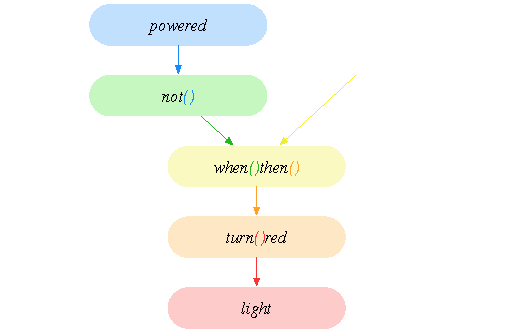
\includegraphics[width=\linewidth,height=\linewidth,keepaspectratio]{figures/example1comp.pdf}
\caption{The example expression compiled into a directed acyclic graph} 
\label{fig:example1comp}
\end{figure}

This graph representation is in fact Single Static Assignment (SSA) form \cite{cytron91efficiently} of the executable implementing the specified interaction. This form allows different uses such as optimisations, verification, proofs and code generation.

\subsection{Optimisation}

Optimisation can be performed by analysing the graph representation, and generating different execution schemes depending on the requested inputs and outputs, using techniques such as push (data driven evaluation) and pull (demand driven evaluation) as applied to functional reactive programming  in \cite{Elliott:2009:PFR:1596638.1596643}.

\subsection{Verification}

Verification and proof can be performed by transforming intermediate representation into state machines. The graph representation exactly describes the transition function of such a system, while the state vector is easily derived. It is important to note that the only way for data to persist from one execution step to the next is to be part of a \code{previous()} interaction. Hence, the state vector is \emph{exactly} the set of interactions which are included in \code{previous()} interactions. Finally, the generated system has a structure which is very similar to systems generated by other synchronous data flow programming languages such as Scade or Lustre \cite{halbwachs91}. This potentially allows to leverage the verification tools that have been developed and used for these languages.

\subsection{Code generation}

Code generation has two main objectives: prototype code generation, and production code generation. Both are similar in nature, and are made relatively easy thanks to the intermediate representation.  The target languages only have to provide a few features: compound data types, functions, and data types corresponding to LIDL basic data types. At the moment, code generation tools are being developed for two languages: The first is Javascript, in order to enable quick prototyping in a web app, and even some sort of Read-Eval-Print-Loop similar to the one available online for the Elm functional reactive programming language \cite{czaplicki2012elm}. The other target language is C, as it is probably the most common language in use for critical systems.


\subsection{Human models and automatic testing}

We have seen that LIDL can be used to specify interactions to be performed by computers. It is also a surprisingly convenient way to model interactions to be performed by human agents.

The high abstraction capabilities of LIDL coupled with its close-to-natural-language syntax allows to specify human interactions associated with a system in a very formal way, while remaining similar to a user manual. LIDL descriptions of human interactions are interesting because they bridge the gap between \emph{task models} and \emph{user manuals} \cite{Bowen:2012:MUM:2305484.2305505}, being a generalisation of both.

Typically, LIDL developers would code two things: computer-side interactions (e.g a widget behaviour), and their human-side counterparts (e.g. how to use a widget). This approach is similar to test driven development, applied to interactive systems. This formal specification of human interactions enables automatic testing, by executing a system composed of the computer-side interactions on one side, and the human-side interaction on the other, in an approach similar to \cite{Barboni:2010:BMI:1822018.1822043}.

Furthermore, LIDL makes it easy to take into account and model human errors and non deterministic behaviour such as those detailed in \cite{bolton2011} and \cite{martinie2014fine}. This allows to test interactive systems even more completely, by simulating the consequences of human errors. Listing \ref{examplehuman} shows an example human-side interaction that details how to click on a button, taking into account one error type: omission. The \code{either()()} interaction represents a non-deterministic choice.


\begin{lstlisting}[caption=LIDL definition of a potentially faulty human interaction,label=examplehuman]
interaction
  (click on (theButton: Button)): Activation in
is
  ( either 
    ((theButton.click)=(active))   // Nominal
    (nothing)                      // Omission !
  )
\end{lstlisting}







%%%%%%%%%%%%%%%%%%%%%%%%%%%%%%%%%%%%%%%%%%%%%%%%%%%%%%%%%%%%%%%%%%%
\section{Use case}

In this section, we will use LIDL to describe parts of a user interface. The user interface in question allows to control the Boiling Water Reactor (BWR) of a nuclear power plant. For the sake of simplicity, we will limit ourselves to an abstract interface as described in \cite{Paterno:2009:MUD:1614390.1614394}. However, LIDL is not restricted to the specification of abstract user interfaces.

LIDL puts an emphasis on reusability. In the use case, this means that we will take advantage of the similarities between components in order to limit the bulk of code. Figure \ref{fig:screenshot} shows common elements in coloured frames, these common elements will be coded as reusable components.

\begin{figure}[h]
\centering
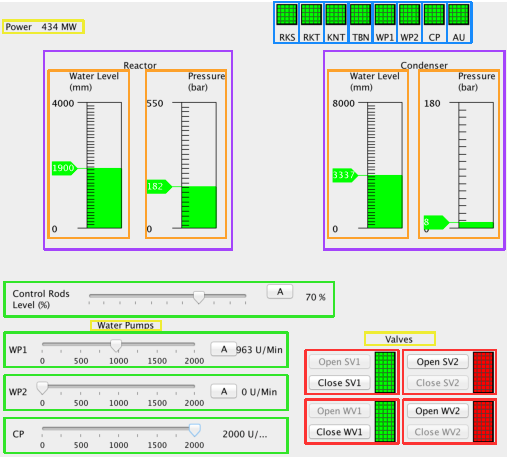
\includegraphics[width=\linewidth,height=\linewidth,keepaspectratio]{figures/screenshot.pdf}
\caption{A screenshot of the BWR simulator with some common elements outlined in common colors} 
\label{fig:screenshot}
\end{figure}



\subsection{LIDL implementation of a basic component}

To get started, let's look at the implementation of a simple abstract slider, which could be part of a standard abstract widget library for LIDL.



Listing \ref{sliderinterface} shows the interface that this abstract slider complies to. The abstract slider outputs two things to the user: The value of the slider, concretely implemented by the position of the cursor, and the slider range, concretely implemented by the labels at each end of the slider. The abstract slider has one input from the user: The position that the user wants the slider to be at. 


\begin{lstlisting}[caption=The interface of an abstract slider,label=sliderinterface]
interface Slider is
  {
    value: Number out,
    range: {min: Number, max: Number} out,
    selection: Number in
  }
\end{lstlisting}


We could define many interactions that implement this interface. Listing \ref{sliderinteraction} presents one of them. This implementation follows these arbitrary design choices:

\begin{itemize}
  \item It takes an \code{enabled} argument that specifies if the slider is enabled or not.
  \item It takes two arguments to specify the range of the slider.
  \item In case no value is provided for the slider position, it will initialise as the lower bound of the range.
  \item It sets the value of the argument \code{theSelection} when changed by the user, or when the range is changed so that it becomes incompatible with the previous value of the slider.
  \item It take an argument \code{constrainedPosition} that allows to programatically set the value of the slider, overriding user input.
\end{itemize}

Several interactions are used in order to define the slider interaction. For example, note the use of the \code{()fallbackto()fallbackto...} interaction (lines 16-19). This interaction uses the activation of its arguments, and picks the first argument which is active.

Another important point to notice is the argument named \code{theSelection} (line 5). Since it is an \code{out}, it will not be read in order to compute a result. In fact, it will be written to, i.e. a value will be sent to it. This is unlike other arguments that are \code{in}, which have roles similar to arguments programmers are used to.

By looking at this implementation of the slider, it is really easy to notice that it is a stateful component. Indeed we can see a \code{previous()} interaction (line 18). The interaction inside the \code{previous()} is \code{currentValue}, so \code{currentValue} is the state variable.

\begin{lstlisting}[caption=The definition of an abstract slider interaction,label=sliderinteraction]
interaction 
  ( slider (enabled: Activation in)
    between (min:Number in) and (max:Number in)
    constrained to (constrainedPosition: Number in)
    selecting (theSelection: Number out)
  ): Slider
is
  ((when (enabled) 
    then ({
      value:(currentValue),
      range:({min:(min),max:(max)}),
      selection:(userInput)
    }))
   behaviour 
    ((current value)=
      (((constrainedPosition)
        fallback to (userInput) 
        fallback to (previous(currentValue)) 
        fallback to (min))
      kept between (min) and (max))
    ))
with
  interaction (currentValue):Number ref
  interaction (userInput):Number ref
\end{lstlisting}


Listing \ref{sliderinstance} shows an example use of the slider defined in Listing \ref{sliderinteraction}. This instance will always be enabled, because the \code{enabled} argument is set to the constant \code{active}. Since the constrained value is set to \code{inactive}, this instance will allow the user to select a number in the constant range $[0,2000]$, and the value selected by the user will be sent to a variable named \code{myValue}.


\begin{lstlisting}[caption=An instance of the abstract slider,label=sliderinstance]
(slider (active) between (0) and (2000) 
  constrained to (inactive) selecting (myValue))
\end{lstlisting}


\subsection{LIDL implementation of a compound component}


We will describe the components framed in green on Figure \ref{fig:screenshot}. These components, that we will call ``complex sliders'', are composed of:

\begin{itemize}
  \item A \textcolor{c0}{label} indicating the purpose of the slider to the user 
  \item A \textcolor{c3}{slider} allowing the user to select a value. The slider is the one defined in the previous section 
  \item A \textcolor{c6}{toggle button} to switch between manual and auto modes 
  \item A \textcolor{c9}{label} indicating the value and units of the selection 
\end{itemize}


\begin{figure}[h]
\centering
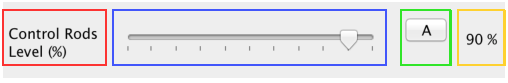
\includegraphics[width=\linewidth,height=\linewidth,keepaspectratio]{figures/screenshotSlider.pdf}
\caption{A screenshot of a complex slider component} 
\label{fig:screenshotSlider}
\end{figure}

Figure \ref{fig:screenshotSlider} shows the concrete implementation of this complex slider, and Listing \ref{complexinterface} shows its LIDL interface. Note that it reuses the \code{Slider} interface defined in the previous section, as well as other interfaces. 

\begin{lstlisting}[caption=The interface of the complex slider,label=complexinterface]
interface ComplexSlider is
  {
    title: Label,
    slider: Slider,
    toggle: ToggleButton,
    value: Label
  }
\end{lstlisting}

Listing \ref{complexinteraction} shows an implementation of this complex slider. 

\begin{lstlisting}[caption=Definition of a complex slider interaction,label=complexinteraction]
interaction ( 
  complex slider
  named (title: Text in)
  between (min:Number in) and (max:Number in) 
  (units:Text in)
  constrained to (constrainedPosition: Number in)
  selecting (theSelection: Number out)
  requesting (mode: Activation out) automation
  ):ComplexSlider
is
  ({
    title: (
      label (active) 
      displaying (title)),
    slider: (
      slider (active) 
      between (min) and (max) 
      constrained to (constrainedPosition)
      selecting (theSelection)),
    toggle: ( 
      toggle (active) 
      pushed (when(constrainedPosition)) 
      displaying ("A") 
      toggling (mode)),
    value: (
      label (active) 
      displaying ((theSelection) " " (units)) )
  })
\end{lstlisting}

Listing \ref{complexinstance} shows an example instance of this complex slider, corresponding to the concrete implementation depicted in Figure \ref{fig:screenshotSlider}.

\begin{lstlisting}[caption=An instance of the complex slider interaction,label=complexinstance]
( complex slider
  named ("Control Rods Level")
  between (0) and (100) ("%")
  constrained to (controlRodsAutoValue)
  selecting (controlRodsLevel)
  requesting (controlRodsAutoMode) automation
)
\end{lstlisting}

\section{Conclusion}

This paper presented a quick overview of LIDL, a language dedicated to the description of interactions, and a use case. The use case showed that LIDL allows to specify safe complex behaviour. In particular, it is noteworthy that, as compared to other approaches, the LIDL way of thinking as two consequences: 
\begin{itemize}
  \item Removing duplicate or boilerplate code as seen in other languages, such as getter/setters and observer pattern functions. This is noticeable by the relatively small size of LIDL programs.
  \item Forcing designers into thinking about the actual interaction, enforcing to explicitly define aspects that are usually implicit or merged into objects whose semantics are not clear. This is noticeable in the slider example (Listing \ref{sliderinteraction}), where an explicit distinction is made between the user input and the slider current value. This explicit distinction allows to have a sane behaviour, even when the slider range is dynamically changed, while keeping the code simple.
\end{itemize} 

 LIDL is only a language. Architectural concepts that fit with LIDL are being developed, but not detailled in this paper. The architectural ideas behind LIDL converge with those recently presented in \cite{facebook-react} and similar approaches around uni-directional data flow. A general framework for the specification of abstraction levels of interactive systems inspired by \cite{Zave:2012:GVN:2405178.2405179} is being developed in parallel with LIDL.


%\appendix
%\section{Appendix Title}
%
%This is the text of the appendix, if you need one.
%
%\acks
%
%Acknowledgments, if needed.

% We recommend abbrvnat bibliography style.

\bibliographystyle{abbrvnat}

% The bibliography should be embedded for final submission.

\bibliography{bibliography.bib}


\end{document}

%                       Revision History
%                       -------- -------
%  Date         Person  Ver.    Change
%  ----         ------  ----    ------

%  2013.06.29   TU      0.1--4  comments on permission/copyright notices

